\documentclass[a4paper,10pt]{article}
\usepackage[utf8]{inputenc}
\usepackage{polski}
\usepackage{graphicx}
\usepackage{listings}
\usepackage[usenames,dvipsnames]{color}
\addtolength{\hoffset}{-1cm}
\addtolength{\voffset}{-2cm}
\addtolength{\textwidth}{2cm}
\addtolength{\textheight}{3cm}
\usepackage{setspace}
\usepackage{indentfirst}
\usepackage{graphicx}
\lstset{
    language=Matlab,
    basicstyle=\scriptsize,
    aboveskip={1.5\baselineskip},
    columns=fixed,
    showstringspaces=false,
    extendedchars=true,
    breaklines=true,
    tabsize=4,
    prebreak = \raisebox{0ex}[0ex][0ex]{\ensuremath{\hookleftarrow}},
    frame=single,
    showtabs=false,
    showspaces=false,
    showstringspaces=false,
    identifierstyle=\ttfamily,
    keywordstyle=\color[rgb]{0,0,1},
    commentstyle=\color[rgb]{0.133,0.545,0.133},
    stringstyle=\color[rgb]{0.627,0.126,0.941},
    numbers=left,
    numberstyle=\tiny,
    stepnumber=1,
    numbersep=5pt,
    captionpos=b,
    escapeinside={\%*}{*)}
}

\def\figurename{Rys.}
\def\lstlistingname{Fun.}

\title{Informatyczne Systemy Sterowania \\ \large Ćwiczenie 3: Regulacja dwu- i trójpołożeniowa}

\author{Adam Jordanek 168139, Tomasz Klimek 168092}

\begin{document}
\maketitle

\section{Wstęp}\label{sec:wstęp}
\subsection{Cel ćwiczenia}
Celem tego ćwiczenia jest symulacja działania systemu regulacji z przekaźnikami dwu- i trójpołożeniowymi. Ćwiczenie umożliwić zapoznanie się z nieliniowymi algorytmami sterowania (przełącznikami dwu- i trójpołożeniowymi) oraz zapoznanie się ze środowiskiem Simulink oraz Matlab w zakresie nieliniowych algorytmów sterowania.
%Czy to jest dobrze?

\subsection{Plan badań} 
\begin{enumerate}
	\item Symulacja systemu regulacji. Dobór parametrów regulatora. \newline
	%czy to jest poprawne gramatycznie? :P
	 \small {W trakcie realizacji zadania należy zasymulować działanie systemu regulacji pracującego z regulatorem oraz należy zbadać wpływ wartości parametrów przekaźników na przebieg błędu regulacji}
	\begin{enumerate}
		\item Regulator dwupołożeniowy bez histerezy.
		\item Regulator dwupołożeniowy z histerezą.
		\item Regulator trójpołożeniowy bez histerezy.
		\item Regulator trójpołożeniowy z histerezą.
 	\end{enumerate}
	\item Zastosowanie członów korekcyjnych.
	\begin{enumerate}
		\item Modyfikacja systemów z zadania 1 o korekcję w postaci członu liniowego o transmitancji: 
			\begin{equation} \label{eqn:czlonKorekcyjny}
				K_{k}(s) = {k_{k}} \over {T_{k}s+1}
			\end{equation}
		\item Doświadczalny dobor parametrów członu korekcyjnego.
	\end{enumerate}
\end{enumerate}

\newpage
\section{Realizacja planu i wyniki}
%---------------------------------------------------------------------------------------------------------------------
%ZADANIE 1
%---------------------------------------------------------------------------------------------------------------------
\subsection{Symulacja systemu regulacji. Dobór parametrów regulatora.}\label{sec:zad1}
% TU DODAĆ JAKIŚ UGÓLNY WSTĘP
\subsubsection{Regulator dwupołożeniowy bez histerezy}\label{sec:r2bh}
\begin{figure}[h]
    \centering
	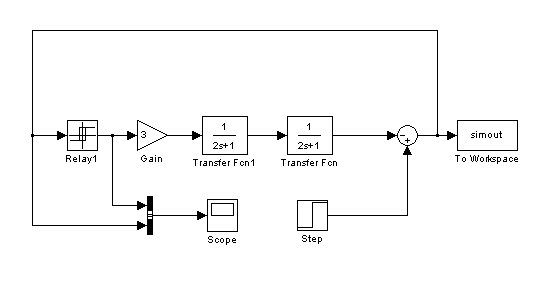
\includegraphics[width=120mm]{CW3-schemat-2bez.png}
	\caption{Schemat symulacji regulatora dwupołożeniowego bez histerezy}
    \label{fig:Rysunek}
\end{figure}

\begin{figure}[h]
    \centering
	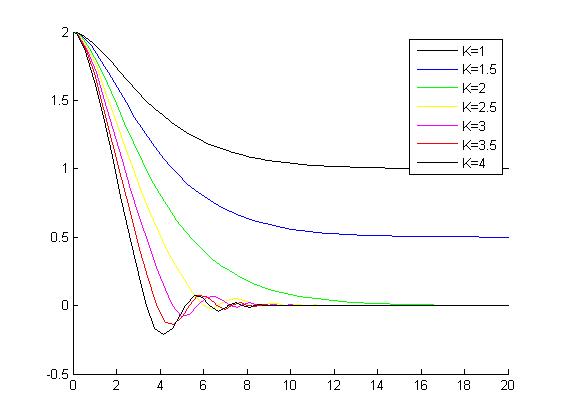
\includegraphics[width=120mm]{CW3-wykres-2bez.png}
	\caption{}
    \label{fig:Rysunek}
\end{figure}

\subsubsection{Regulator dwupołożeniowy z histerezą}\label{sec:r2h}
\begin{figure}[h]
    \centering
	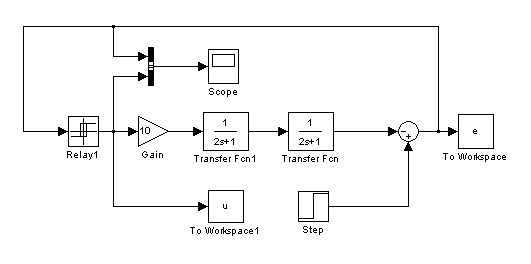
\includegraphics[width=120mm]{CW3-schemat-2z.png}
	\caption{Schemat symulacji regulatora dwupołożeniowego z histerezy}
    \label{fig:Rysunek}
\end{figure}

\subsubsection{Regulator trójpołożeniowy bez histerezą}\label{sec:r3bh}

\subsubsection{Regulator trójpołożeniowy z histerezą}\label{sec:r3h}
%---------------------------------------------------------------------------------------------------------------------
%ZADANIE 2
%---------------------------------------------------------------------------------------------------------------------
\subsection{Zastosowanie członów korekcyjnych.}\label{sec:zad2}
\subsubsection{Modyfikacja systemów z zadania 1}\label{sec:zad2_1}
\subsubsection{Doświadczalny dobor parametrów członu korekcyjnego.}\label{sec:zad2_2}

\end{document}